\documentclass[a4paper]{article}

\usepackage[utf8]{inputenc}
\usepackage{graphicx}
\usepackage{float}
\usepackage[caption = false]{subfig}
\usepackage{amsmath}
\usepackage{indentfirst}
\usepackage{hyperref}
\usepackage[margin=2.8cm]{geometry}
\usepackage{ragged2e}
\usepackage{makecell}
\usepackage{multirow}
\usepackage{bm}

\title{Clustering Molecular Structures for Next-generation Solar Cell Material Discovery}
\author{Gustave Li}
\date{August 24, 2021}

\begin{document}

\maketitle

\section{Abstract}

\section{Introduction}
The Carotenoid-Porphyrin-\(\text{C}_{60}\) (\(\text{CPC}_{60}\)) triad molecule consists of a porphyrin covalently linked with a carotenoid and a \(\text{C}_{60}\) molecule (Figure~\ref{fig:CPC60}). Carotenoid is the excited-state electron donor and the \(\text{C}_{60}\) serves as the electron acceptor, while porphyrin acts as a bridge to separate the two parts and transfer electrons. The molecule is a mimicry of the natural photosynthetic center which utilize photons to initiate a complex series of electronic transitions to achieve a high-energy charge separated state. It absorbs UV visible light and produces a charge separated state (\(\text{CT}_{2}\)) where an electron is transferred from C to \(\text{C}_{60}\), producing a large dipole moment of 150 D. Due to its outstanding performance in photoinduced charge transfer, it has a great potential in organic solar cells.

However, Manna et al. reported that the triad spatial conformation strongly affects the process of charge separation and concluded that the linear conformations have better charge separation effeciency over the bent conformations \cite{MannaArun}. Olguin et al. further investigated the effect of structural changes on \(\text{CPC}_{60}\) charge transfer states, they summarized several factors influencing charge transfer, including donor-acceptor distance, distances and torsions between the three components \cite{OlguinMarco}. In summary, the charge transfer process in \(\text{CPC}_{60}\) is very conformation-dependent,  the molecular structure has a rather dramatic effect on the the charge transfer performance. Thus, finding the optimal structure for charge transfer is critical.

\begin{figure}[H]
    \centering
    \subfloat[Linear]{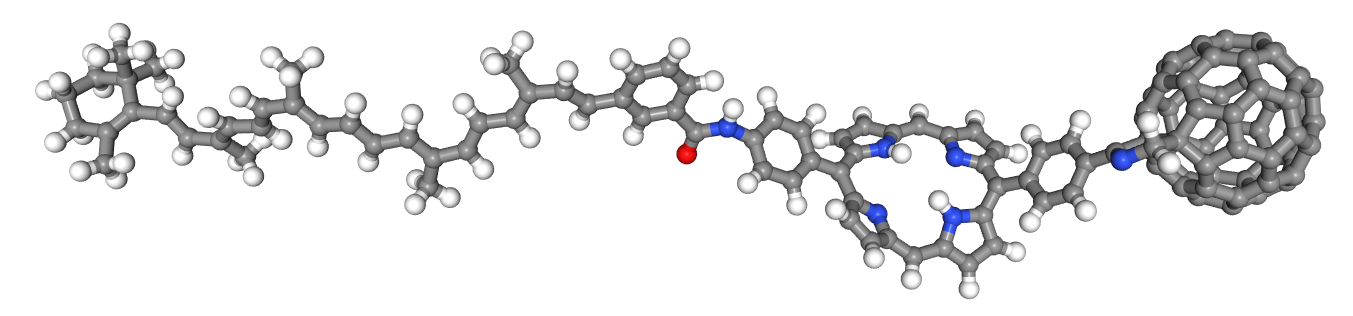
\includegraphics[width=0.4\linewidth]{projects/Gustave_Li/Docs/pics/Triad_linear.png}}
    \subfloat[Bent]{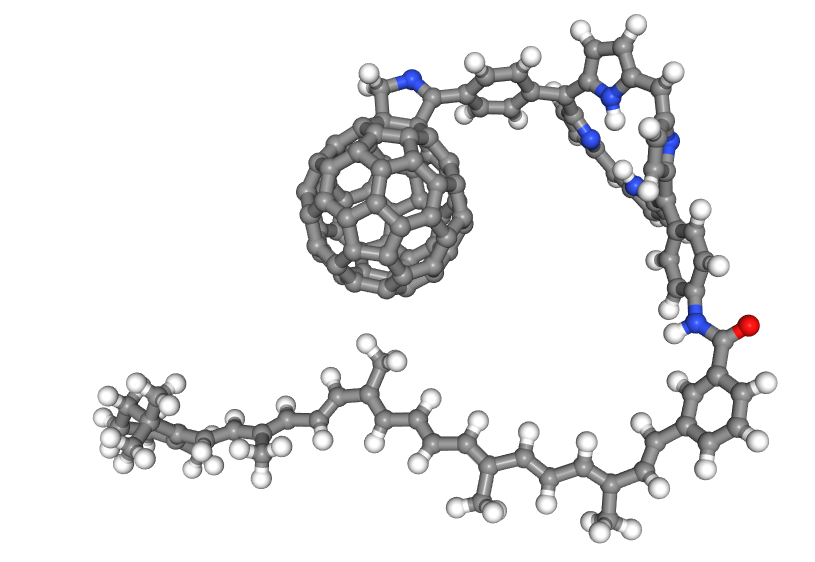
\includegraphics[width=0.3\linewidth]{projects/Gustave_Li/Docs/pics/Triad_bent.png}}
    \caption{Different conformations of \(\text{CPC}_{60}\) molecule}
    \label{fig:CPC60}
\end{figure}

Thanks to the development of computer sciences, tens of thousands of possible \(\text{CPC}_{60}\) molecules can be generated based on molecular dynamics. Considering the heavy computing load of calculation and the complexity of the \(\text{CPC}_{60}\) molecule, it is unrealistic to calculate the charge transfer rate for all the molecules. Researchers are currently working on different directions to address this issue. Brian and co-worker proposed novel formulations for calculating charge transfer rate, which reduced a maximum of 80\% of computational cost \cite{BrianDomi}. In this project, we aim to make use of machine learning to cluster the many molecules into different groups, and explore the possible machine learning pipeline that is suitable for the triad-molecule clustering scenario. By taking the cluster center as representation conformations, we expect the computational cost to decrease for a great amount while maintaining as much structural information as possible.

\section{Tools \& Platforms}

The tools and platforms used in this project are listed in Table \ref{table: tools & platforms}. Additionally, different python modules are implemented to accomplish various tasks throughout the project (see detailed information in Table \ref{table: python modules}). All the python codes and results can be found under the GitHub repository: \href{https://github.com/xiangsunlab/durf_hq/tree/master/projects/Gustave_Li}{github.com/xiangsunlab/durf\_hq/tree/master/projects/Gustave\_Li}.

\begin{table}[h!]
    \centering
    \caption{Tools and platforms used in the project} 
    \begin{tabular}{l|l}
    \hline \hline
        \textbf{Tools / Platforms} & \textbf{Description} \\
        \hline
        Python & Major programming language \\
        Markdown & Light-weight note-taking language \\
        Jupyter Notebook \& Spyder & Code experiment \& module management \\
        GitHub & Project management \\
        Overleaf & Documentation \& this report \\
        NYUSH HPC & Computing resources \\
        \hline \hline
    \end{tabular}
    \label{table: tools & platforms}
\end{table}

\begin{table}[H]
    \centering
    \caption{Python modules}
    \begin{tabular}{l|l}
    \hline \hline
        \textbf{Python modules} & \textbf{Description} \\
        \hline
        Numpy, Pandas & Data processing \\
        MDTraj\cite{MDTraj}, MDAnalysis\cite{MDAnalysis_1}\cite{MDAnalysis_2}, PyEMMA \cite{pyemma}     & Triad data reading \& analysis \\
        NGLview\cite{NGLview} & Triad molecule visualization \\
        Scikit-learn\cite{scikit-learn}, sklearn\_extra, hdbscan\cite{hdbscan} & Machine learning algorithms \\
        Matplotlib, Bokeh & Plotting \\
        \hline \hline
    \end{tabular}
    \label{table: python modules}
\end{table}

\section{Experiment Methods}

\subsection{General Workflow}
The original dataset is a molecular dynamics file containing 100,000 frames of the triad molecule. The data was first visualized to obtain basic structure and chemical features of the triad molecules. Two feature spaces were prepared for machine learning process: \textbf{a)} the xyz coordinates of each atom in the triad molecule, \textbf{b)} 8 descriptors (distances, angles, torsions) selected to represent the structure. With the feature space prepared, dimensionality reduction was applied to both spaces via different approaches and the dimensionality was reduced to 2D space for plotting and inspection conveniences. The different reduced-dimensional data were put into various clustering algorithms, which generate cluster centers (core instances) and instance labels. Quality of clustering result was evaluated with multiple criterion and some suboptimal pipelines were eliminated from the following steps. Clustering was then performed once again in the original high-dimensioanl feature space with cluster center pre-determined by the previous 2D clustering methods. Triad molecules were assigned to different clusters based on their structural similarities with core instances. High-dimensional clustering results were inspected and three machine learning methods that produces the best results were chosen.

\subsection{Descriptors}
The xyz coordinates data is the simplest feature space when it comes to describing molecular structures. However, xyz coordinates suffers from several major drawbacks: First of all, the dimension of the dataset is too high. Each triad molecule has 207 atoms with 3 coordinates for each atom, so the total dimension for each entry is 621. Such large dimension may not only take up large memory for computer to store and process the data, but also increase the risk of over fitting caused by the redundant information stored in such large dimension. Secondly, xyz coordinates are orientation sensitive. While the orientation of a single molecule has very limited effect on its chemical properties, the xyz coordinates can be very different when the molecule was translated or rotated. From this point of view, the clustering algorithm will likely to over-estimate the importance of molecular orientation and position, which gives the suboptimal result.

\subsubsection{Key Atoms \& Descriptors List}
With the aim of addressing the pitfalls of xyz data space, descriptors should be concise and not orientation-sensitive. Distances between two ends of the triad describe the overall structure of the molecule, angles and dihedrals represent the bending and twisting of each part of the molecule. RMSD with reference to the bent and linear structure displays the extent of streching and bending. The full descriptors are listed in Table \ref{table: descriptors}. Considering the three-component ( Carotenoid-Porphyrin-\(\text{C}_{60}\))  nature of the molecule and its various structures, the following atoms are chosen as key atoms and all the descriptors are computed based on them: \(\text{C}_{33}\), \(\text{C}_{21}\), \(\text{C}_{61}\), \(\text{C}_{65}\), \(\text{C}_{66}\), \(\text{C}_{69}\), \(\text{C}_{89}\), \(\text{C}_{95}\), \(\text{C}_{96}\), \(\text{C}_{128}\) and \(\text{N}_{6}\) (shown in Figure \ref{fig: key atoms}).

\begin{figure}[H]
    \centering
    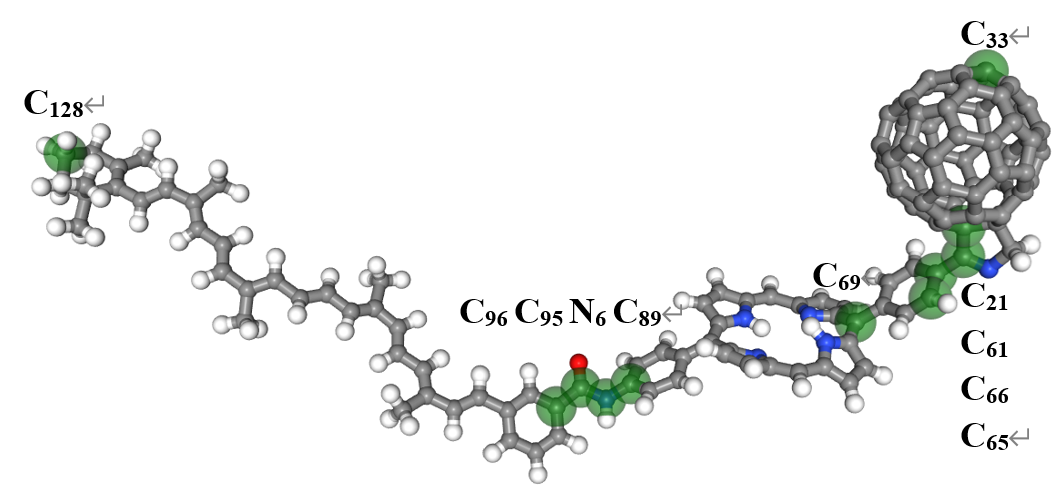
\includegraphics[width=0.75\linewidth]{projects/Gustave_Li/Docs/pics/key_atoms.png}
    \caption{Key atoms for descriptors}
    \label{fig: key atoms}
\end{figure} 

\begin{table}[H]
    \centering
    \caption{Definitions of geometric descriptors}
    \begin{tabular}{l|l}
    \hline \hline
       \textbf{Name}  & \textbf{Description} \\
       \hline
       EuclidianDist\_1 & The euclidian distance between \(\text{C}_{33}\) \& \(\text{C}_{128}\) \\
       Angle\_1 & The angle between atoms \(\text{C}_{33}\)-\(\text{C}_{96}\)-\(\text{C}_{128}\) \\
       Angle\_2 & The angle between atoms \(\text{C}_{33}\)-\(\text{C}_{69}\)-\(\text{C}_{96}\) \\
       Angle\_3 & The angle between atoms \(\text{C}_{69}\)-\(\text{C}_{96}\)-\(\text{C}_{128}\) \\
       Dihedral\_1 & The absolute valute of dihedral between atoms \(\text{C}_{21}\)-\(\text{C}_{61}\)-\(\text{C}_{66}\)-\(\text{C}_{65}\) \\
       Dihedral\_2 & The absolute valute of dihedral between atoms \(\text{C}_{89}\)-\(\text{N}_{6}\)-\(\text{C}_{95}\)-\(\text{C}_{96}\) \\
       RMSD\_Linear & RMSD for the conformation to the Linear triad \\
       RMSD\_Bent & RMSD for the conformation to the Bent triad \\
       \hline \hline
    \end{tabular}
    
    \label{table: descriptors}
    \vspace{1ex}
    {\noindent \justifying Note: the linear and bent conformation was determined by the overall bending angle of the triad molecule, described by the Angle\_1 descriptor. For our triad dataset, we defined the triad indexing 88213 as the linear model, which has an overall angle of \(3.10\,rad\). The bent was defined as the 29685th frame, which has an angle of \(0.36\,rad\). \par}
\end{table}

\subsection{Dimensionality Reduction}
Each of the triad molecules consist of 207 atoms, thus each molecule is represented as a data point in a 621 (\(207 \times 3\)) dimension space. In such high dimensional space, data points are far sparser than that in lower dimensional spaces, thus making it harder to find the optimal clustering result. The difficulty caused by high dimensionality is referred to as \textit{the curse of dimensionality}\cite{GeronAurelien}. Although the dimensionality was reduced to 8 by finding descriptors of the molecular structure, visualization of the 8D descriptors is still unachievable. In the face of such situation, dimensionality reduction plays its role by reducing the dimensionality of dataset significantly (to 2 or 3 for visualization) while preserving the information from original dataset\cite{GlielmoAldo}.

\subsubsection{Dimensioanlity Reduction Methods \& Hyperparameters}
Dimensionality reduction was performed on both xyz feature space and the descriptors space. Linear(PCA) and non-linear(kPCA, tSNE) dimensionality reduction methods were implemented. Hyperparameters were tuned as recorded in Table \ref{table: dimreduct}.

\begin{table}[H]
    \centering
    \caption{Dimensionality reduction method and hyperparameters}
    \begin{tabular}{p{.47\textwidth}|p{.4\textwidth}}
    \hline \hline
        \textbf{Method} & \textbf{Hyperparameters} \\
        \hline
        Principle Component Analysis (PCA) & \texttt{n\_components: 2} \\
        \hline
        kernel Principle Component Analysis (kPCA) & \texttt{n\_components: 2} \par \texttt{kernel: poly, rbf} \\
        \hline
        t-Distributed Stochastic Neighbor Embedding (t-SNE)\cite{KobakDmitry} & \texttt{n\_components: 2} \par \texttt{perplexity: 50} \par \texttt{learning\_rate: (num\_of\_data)/12} \par \texttt{init: pca} \\
        \hline \hline
    \end{tabular}
    \label{table: dimreduct}
\end{table}

\subsubsection{Dimensionality Reduction Results Inspection}
The inspection was achieved by the \texttt{pyemma.plots.plot\_density} module, which plots the dimensionality reduction results on a 2D plane and colors the data points according to the density of that region. Areas that are denser than others are likely to form meaningful clusters.

\subsection{Clustering}
Clustering divides the entire data into several distinct groups, whose elements are similar in the same group and vary between groups \cite{GlielmoAldo}. With the dimensionality reduced feature space prepared, clustering methods were implemented on the low dimensional data.  In order to explore suitable algorithms for triad molecule clustering in a vaster range, different categories of (yet common) clustering algorithms were applied, ranging from kMeans to HDBSCAN. In the meanwhile, different choices of hyperparameters were also explored and evaluated.

\subsubsection{Clustering Methods \& Hyperparameters}

\begin{table}[h!]
    \centering
    \caption{Clustering Methods \& Hyperparameters}
    \begin{tabular}{p{.28\textwidth}|p{.3\textwidth}|p{.3\textwidth}}
    \hline \hline
        \textbf{Category} & \textbf{Method} & \textbf{Hyperparameters} \\
        \hline
        \multirow{2}{.3\textwidth}{Partitioning scheme} & KMeans & \texttt{n\_clusters: 6-10} \\
        & KMedoids & \texttt{n\_clusters: 6-10} \par \texttt{init: k-medoids++} \\
        \hline
        Cluster-density based & Hierarchical density based spatial clustering of applications with noise (HDBSCAN) & \texttt{min\_cluster\_size: 10-100} \par \texttt{min\_samples: 1,10,100} \par \texttt{cluster\_selection\_epsilon: 1,10,100,500} \\
        \hline
        Probability density function & Gaussian mixture model (GMM) & \texttt{n\_components: 6-10} \par \texttt{n\_init: 10} \\
        \hline \hline
    \end{tabular}
    \label{table: clustering methods}
\end{table}

\subsubsection{Clustering Results Inspection}
We have prepared 2 feature spaces, performed dimensionality reduction with 3 methods and implemented 4 clustering algorithms on the data, which is 24 different machine learning combinations (pipelines). For each combination, different hyperparameters also generates different results. With such diversified results, a careful selection is very necessary before moving on to high dimensioanl space. Detailed descriptions of inspection criterion are listed in Table \ref{table: clustering inspection}.

\begin{table}[H]
    \centering
    \caption{Clustering Results Inspection Methods}
    \begin{tabular}{p{.38\textwidth}|p{.6\textwidth}}
    \hline \hline
        \textbf{Methods} & \textbf{Additional notes} \\
        \hline
        Cluster map & \multirow{2}{.6\textwidth}{Provides an intuitive view of how the feature space is divided, and how instances are distributed in each cluster} \\
        Cluster population & \\
        \hline
        Akaike information criterion (AIC) & \multirow{4}{.6\textwidth}{\textbf{a)} AIC and BIC are specific for GMM models, while Inertia is only for KMeans and KMedoids models. \\ \textbf{b)} For comparison and inspection convenience, all the scoring parameters were scaled to range(0,10) before plotting. \\
        \textbf{c)} Scoring evaluates the quality of clustering on a statistical perspective.} \\
        Bayesian information criterion (BIC) & \\
        Inertia & \\
        Silhouette score & \\
          & \\
          & \\
          & \\
        \hline  
        Pairwise RMSD & \multirow{4}{.6\textwidth}{\textbf{a)} The 1000 instances nearest to each cluster center are chosen for pairwise RMSD calculation \\ \textbf{b)} RMSD and Pearson R evaluates the similarity and differences between and within clusters.} \\
        Pearson correlation coefficient & \\
         & \\
         & \\
        \hline \hline
          
    \end{tabular}
    \label{table: clustering inspection}
\end{table}

\paragraph{AIC \& BIC}
AIC and BIC are criterion that select models among a finite set of models, they both introduce penalty for the number of parameters in the model to avoid overfitting \cite{wiki_BIC}. Akaike information criterion is defined as \cite{AIC}:
\begin{equation}
    \text{AIC}=-2\ln(\hat{L})+2k 
    \label{Eq: AIC}
\end{equation}
\noindent where \(k\) is the number of estimated parameters in the model, and \(\hat{L}\) is the maximum value of the likelihood function of the model.

BIC is closely related with AIC and it was derived a little bit later than AIC \cite{BIC}. Formally, Bayesian information criterion is defined as:
\begin{equation}
    \text{BIC}=-2\ln(\hat{L})+k\ln(n)
    \label{Eq: BIC}
\end{equation}
\noindent \(k\) is the number of estimated parameters in the model, \(n\) is the sample size of a certain dataset, and \(\hat{L}\) is the maximum value of the likelihood function of the model.

From the formulae of AIC and BIC, they only differ from their penalty term for model complexity, AIC has penalty form of \(2k\) and BIC is \(k\ln(n)\). The penalty term is larger in BIC than in AIC. Burnham \& Anderson pointed out that AIC can be derived in the same Bayesian framework as BIC, just by using different prior probabilities \cite{AIC_BIC_comparison}\cite{AIC_BIC_book}. Since the likelihood function is negative and the penalty term is positive, the model with lower AIC/BIC is preferred.

\paragraph{Inertia}
Inertia is a criterion that evaluates the cluster coherence generated by KMeans and KMedoids. For a clustering model with \(n\) samples and centroids \(\mu\) in set \(C\), inertia (or within-cluster sum-of-squares criterion) is defined as \cite{scikit-learn}:
\begin{equation}
    \text{Inertia}=\sum_{i=0}^{n}\min_{\mu_{j} \in C} \left( \parallel x_i - \mu_j\parallel^2 \right)
    \label{Eq: inertia}
\end{equation}
\noindent To further explain, inertia calculates the sum of distances between cluster center and each of their cluster members. More compact clusters will result in smaller inertia values, so the model with lower AIC/BIC is preferred.

\paragraph{Silhouette score}
Silhouette score measures how well an instance is inside its own cluster while away from other clusters. It considers both the distance within clusters and distance between different clusters \cite{scikit-learn}:
\begin{equation}
    s = \frac{b-a}{\max(a, b)}
    \label{Eq: Silhouette score}
\end{equation}
\noindent \(a\) is the mean distance between a sample and all other points in the same cluster, and \(b\) represents the mean distance between a sample and all other points in the next nearest cluster. A higher Silhouette Coefficient score relates to a model with better defined clusters. 

\paragraph{RMSD}
Root mean square deviation \( \rho(t) \) is a function that measures atom-wise difference and it can represent structure similarity. The RMSD as a function of time is calculated as:
\begin{equation}
    \rho(t)=\sqrt{\frac{1}{N}\sum_{i=1}^N\left(\bm{x}_i(t)-\bm{x}_i^\text{ref}\right)^2}
    \label{Eq: RMSD}
\end{equation}
\noindent where \(t\) is the time frame and \(N\) is the number of coordinates. It is the Euclidean distance in configuration space of the current configuration (possibly after optimal translation and rotation) from a reference configuration divided by \(\frac{1}{\sqrt{N}}\) \cite{scikit-learn}.

\paragraph{Pearson correlation coefficient}
Pearson correlation coefficient, or Pearson's \( \bm{r}\), gives a quantitative description of similarities between clusters. Given a paired data \(\{(\bm{x}_1, \bm{y}_1), ..., (\bm{x}_n, \bm{y}_n)\}\) consisting of \(n\) pairs, Pearson's \( \bm{r}\) is defined as:
\begin{equation}
    r_{xy} = \frac{\sum_{i=1}^n(x_i-\overline{x})(y_i-\overline{y})}{\sqrt{\sum_{i=1}^n(x_i-\overline{x})^2}\sqrt{\sum_{i=1}^n(y_i-\overline{y})^2}}
    \label{Eq: Pearson R}
\end{equation}
\noindent where \(\overline{x}, \overline{y}\) is the sample mean of \(x\) \& \(y\). Pearson's R first centers the data and returns the cosine of the angle \(\theta\) between the two observed vectors in N-dimensional space, which ranges from -1 to 1 \cite{PearsonR}. Since the triad data is not sensitive to the pointing direction, \(r_{xy}\) closer to 0 shows two clusters are different while a value approaching to -1 or 1 indicates the high similarity between clusters. 

\subsection{High-dimensioanl Clustering}
Although clustering in the 2D reduced space will also generate labels for instances, information is lost when the dimensionality is reduced, raising the risk of membership errors. To ensure the structure information be preserved to its maximum, cluster centers were obtained by clustering in 2D space and cluster members were assigned in the high-dimensional feature space, which make use of RMSD to determine membership. A triad molecule that has RMSD smaller than a given threshold (set to 0.3-0.5), with respect to a cluster center, will be regarded as a member of that cluster. Instances that belong to none of the clusters are treated as exceptions. 

The results are inspected by cluster maps and cluster populations. 

\section{Results \& Discussion}

\subsection{Dimensionality Reduction}
The density map for dimensioanlity reduction results were showed in Figure \ref{fig: dimreduct} \& Figure \ref{fig: dimreduct_xyz}. The color of datapoints represents density. Higher-density region was plotting in yellow and lower-density region plotted in dark purple.

\begin{figure}[H]
    \centering
    \subfloat[PCA]{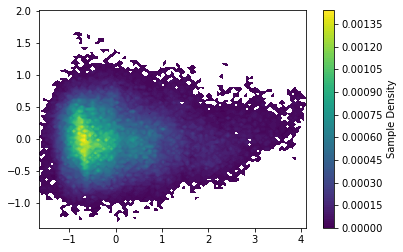
\includegraphics[width=.45\linewidth]{projects/Gustave_Li/Docs/pics/dimreduct/pca.png}}
    \subfloat[kPCA\_poly]{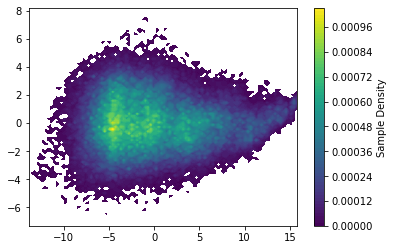
\includegraphics[width=.45\linewidth]{projects/Gustave_Li/Docs/pics/dimreduct/kpca_poly.png}} \\
    \subfloat[kPCA\_rbf]{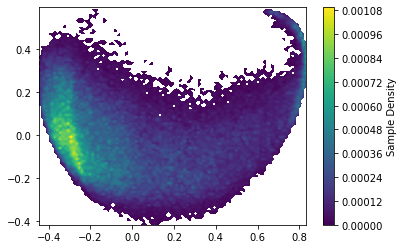
\includegraphics[width=.45\linewidth]{projects/Gustave_Li/Docs/pics/dimreduct/kpca_rbf.png}}
    \subfloat[tSNE]{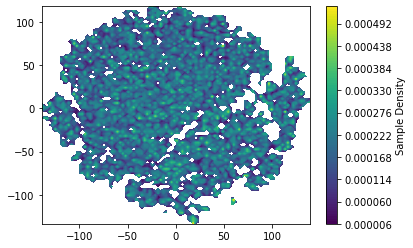
\includegraphics[width=.45\linewidth]{projects/Gustave_Li/Docs/pics/dimreduct/tsne.png}}
    \caption{Dimensionality reduction on descriptors feature space}
    \label{fig: dimreduct}
\end{figure}

\begin{figure}[H]
    \centering
    \subfloat[PCA\_xyz]{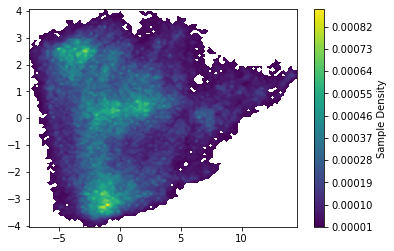
\includegraphics[width=.45\linewidth]{projects/Gustave_Li/Docs/pics/dimreduct/pca_xyz.png}}
    \subfloat[kPCA\_poly\_xyz]{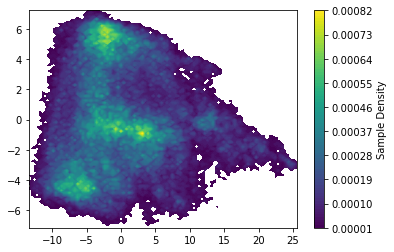
\includegraphics[width=.45\linewidth]{projects/Gustave_Li/Docs/pics/dimreduct/kpca_poly_xyz.png}} \\
    \subfloat[kPCA\_rbf\_xyz]{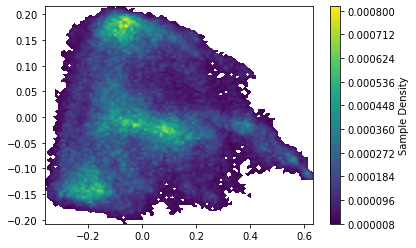
\includegraphics[width=.45\linewidth]{projects/Gustave_Li/Docs/pics/dimreduct/kpca_rbf_xyz.png}}
    \subfloat[tSNE\_xyz]{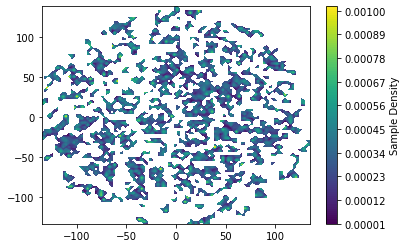
\includegraphics[width=.45\linewidth]{projects/Gustave_Li/Docs/pics/dimreduct/tsne_xyz.png}}
    \caption{Dimensionality reduction on xyz feature space}
    \label{fig: dimreduct_xyz}
\end{figure}

From the two figures, dimensioanlity reduced data was distributed in various shapes with different density. Empirically, clusters forms when high density regions were separated by low density regions (or regions without any instances). This was clearly the case for Figure \ref{fig: dimreduct_xyz}, where multiple yellow regions were surrounded by purple. However, in Figure \ref{fig: dimreduct} (a) (b) (c), the high-density region was continuous without visible low-density area in between. Data represented in Figure \ref{fig: dimreduct} (a) (b) (c) implies that all the data concentrates in one region in the reduced space, i.e., the data only forms one cluster while leaving the rest of the space sparsely filled with data. From the dimensioanlity reduction results, the xyz feature space is expected to behave better in the clustering process.

It can also be found that Figure \ref{fig: dimreduct} (a) (b) has very similar overall shape and density distribution, and analogously for \ref{fig: dimreduct_xyz} (b) (c). Since clustering algorithms works on the relative distribution of data points instead of the absolute coordinates, it is reasonable to choose one of the dimensionality reduction methods that gives similar results, for the next clustering step. Considering both the density distribution and results similarity, kPCA with rbf kernel was left out and reduced data by PCA, kPCA\_poly and tSNE on both descriptor space and xyz space will be put to clustering algorithms.

\subsection{Clustering}

\subsubsection{Cluster Map}
Cluster map gives an intuitive view of the different clusters and cluster centers, it is the most direct method to evaluate cluster quality. An optimal clustering method was expected to give a cluster map that has a moderate number of clusters with cluster member around a certain center. 
\begin{figure}[H]
    \centering
    \subfloat[Eps:1, MinClusterSize:10, MinSample:1]{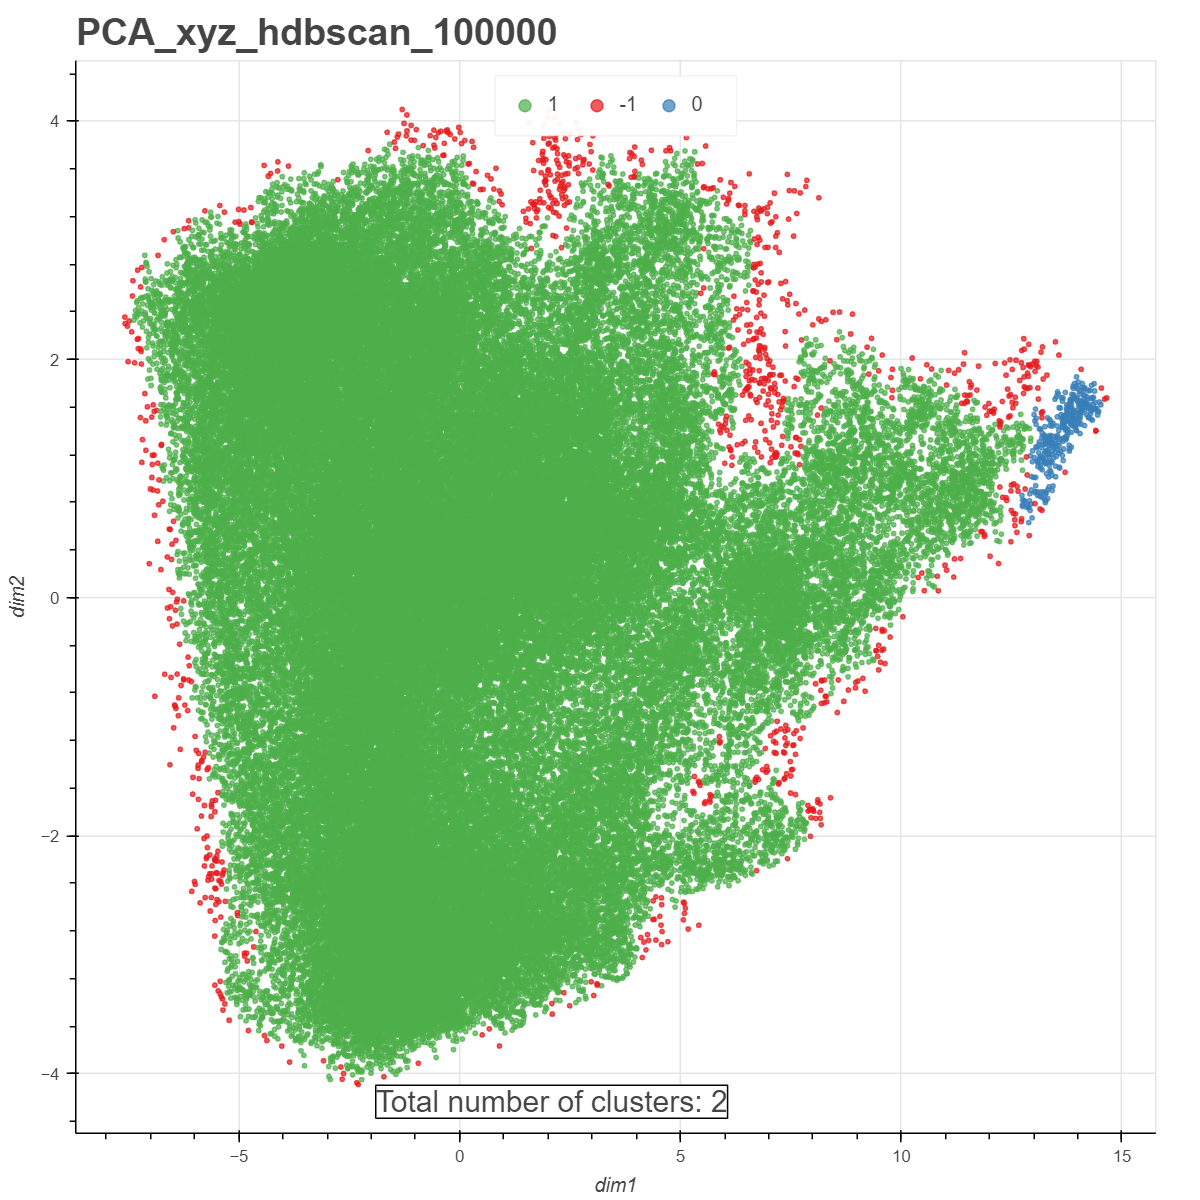
\includegraphics[width=.45\linewidth]{projects/Gustave_Li/Docs/pics/Clustering/Cluster_map/hdbscan_0.png}}
    \subfloat[Eps:1, MinClusterSize:10, MinSample:1]{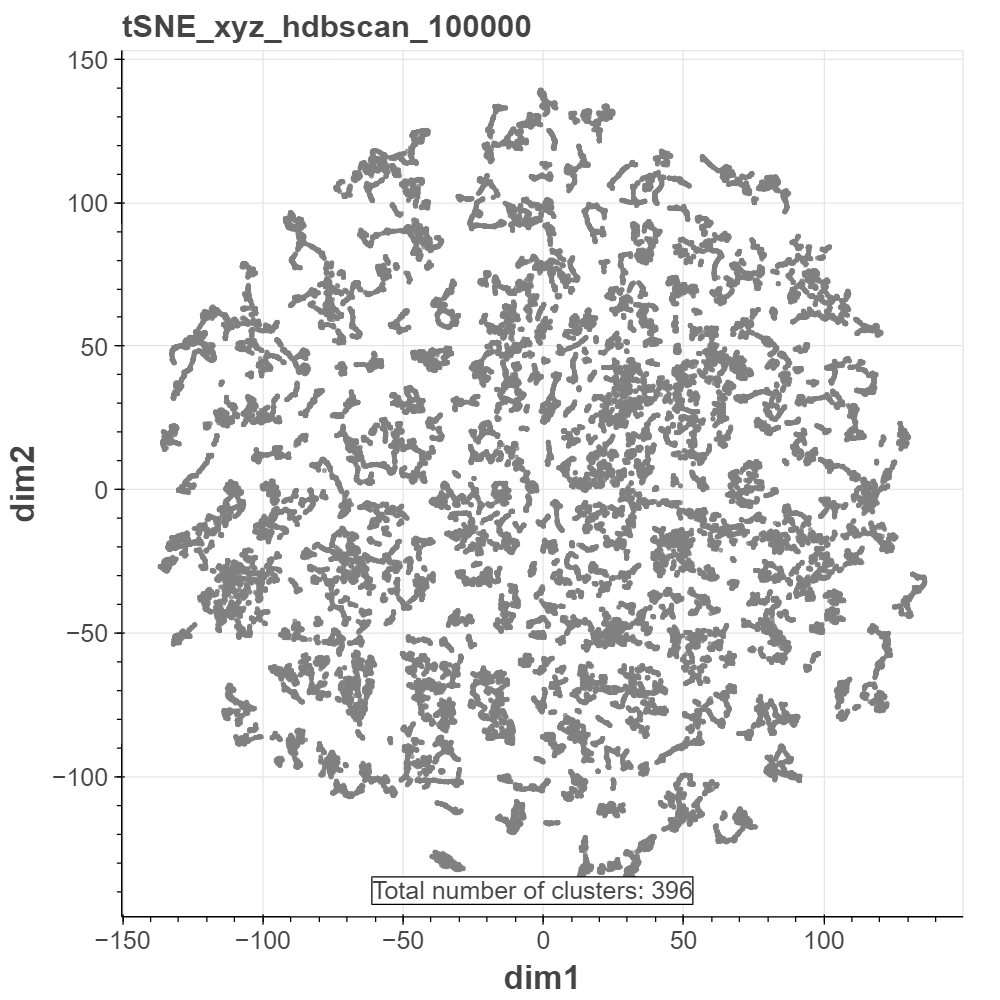
\includegraphics[width=.45\linewidth]{projects/Gustave_Li/Docs/pics/Clustering/Cluster_map/hdbscan_1.png}}
    \caption{HDBSCAN failure}
    \label{fig: HDBSCAN failure}
\end{figure}
After inspecting all the cases generated by HDBSCAN, it failed to meet the basic requirements of an optimum clustering results. Some typical failures are displayed in Figure \ref{fig: HDBSCAN failure}. When processing the triad data, HDBSCAN goes to two extreme: producing too many or too little clusters, and the cluster size varies greatly. HDBSCAN is ruled out from the possible methods for triad clustering.

It is assumed that the failure of HDBSCAN is caused by the nature of the triad data. The working mechanism for HDBSCAN is to find core instances and calculate neighbors of core instances, which is highly dependent to the cluster density. According to the density plots (Figure \ref{fig: dimreduct} \& Figure \ref{fig: dimreduct_xyz}), the density difference is very small between the denser region and the sparser region ((a) (b) (c)), which causes HDBSCAN to divide the whole part as one cluster. As for data generated by tSNE ((d)), the data gets too scattered and HDBSCAN assigned cluster to each of the single pieces, resulting in the algorithm to generate too many clusters.

Unlike HDBSCAN, the cluster numbers generated by KMeans, KMedoids, GMM is pre-determined, thus eliminating the probability of unreasonable cluster numbers. The results generated are quite evenly distributed in the reduced dimensioanl space (examples shown in Figure \ref{fig: clustering PCA} \& Figure \ref{fig: clustering tSNE}).

\begin{figure}[H]
    \centering
    \subfloat[KMeans]{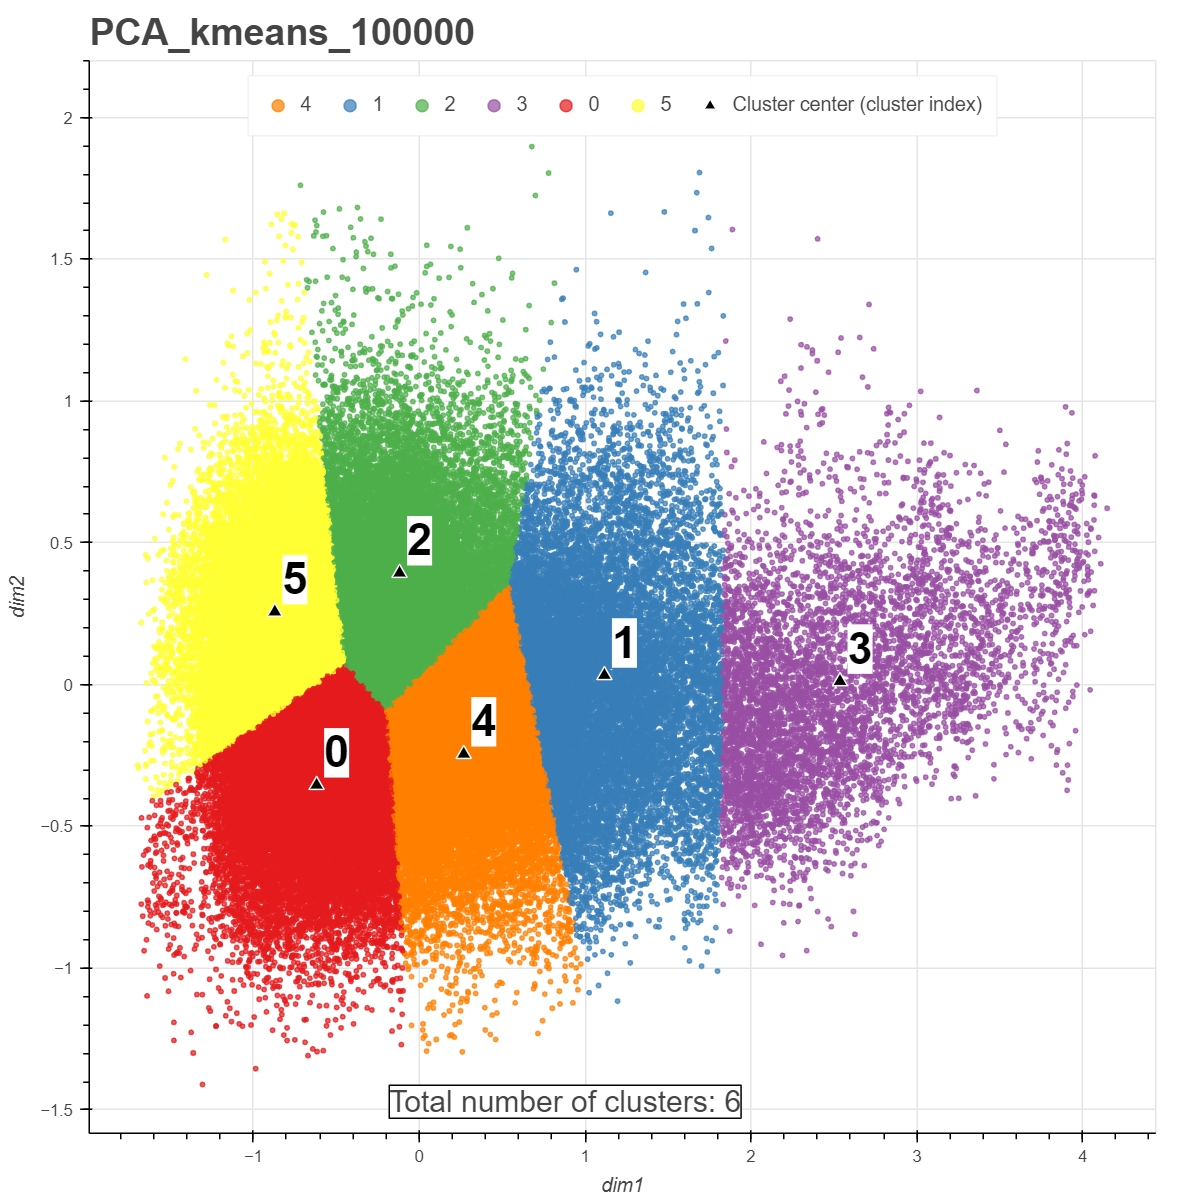
\includegraphics[width=.3\textwidth]{projects/Gustave_Li/Docs/pics/Clustering/Cluster_map/PCA_kmeans.png}}
    \subfloat[KMedoids]{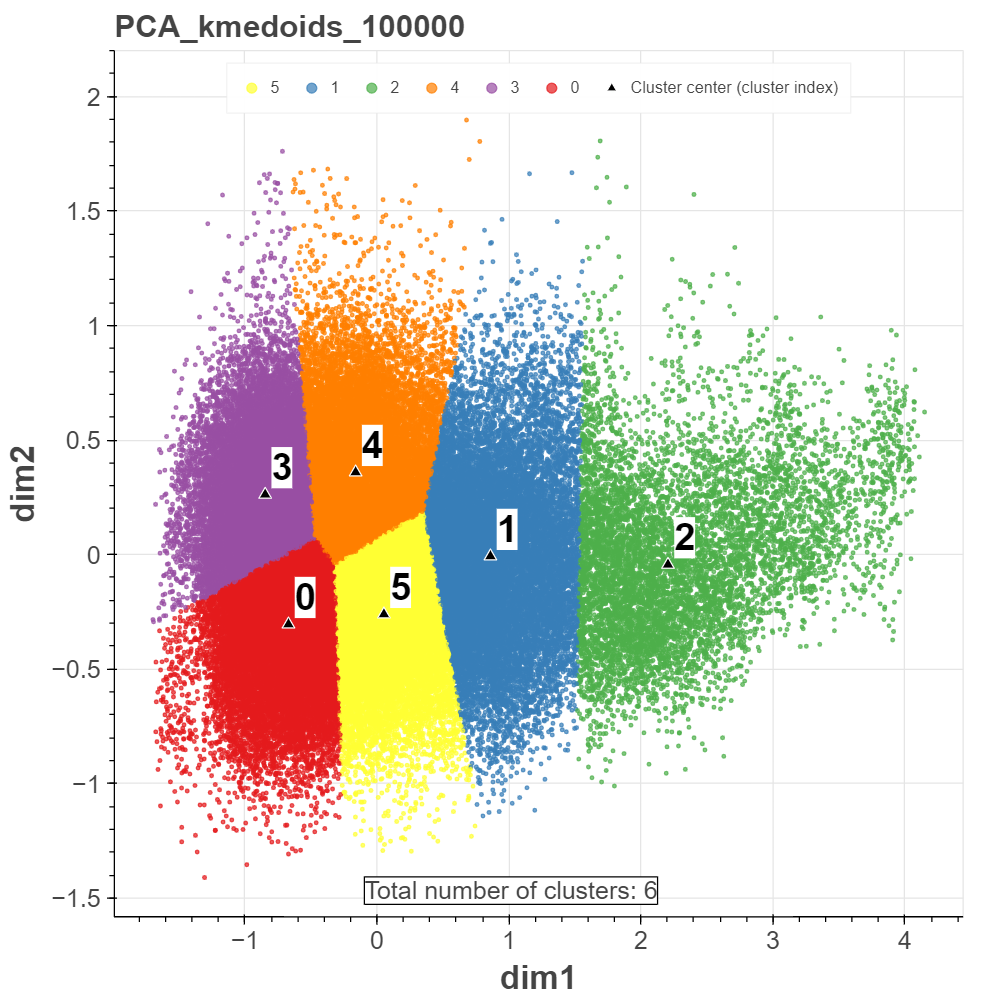
\includegraphics[width=.3\textwidth]{projects/Gustave_Li/Docs/pics/Clustering/Cluster_map/PCA_kmedoids.png}}
    \subfloat[GMM]{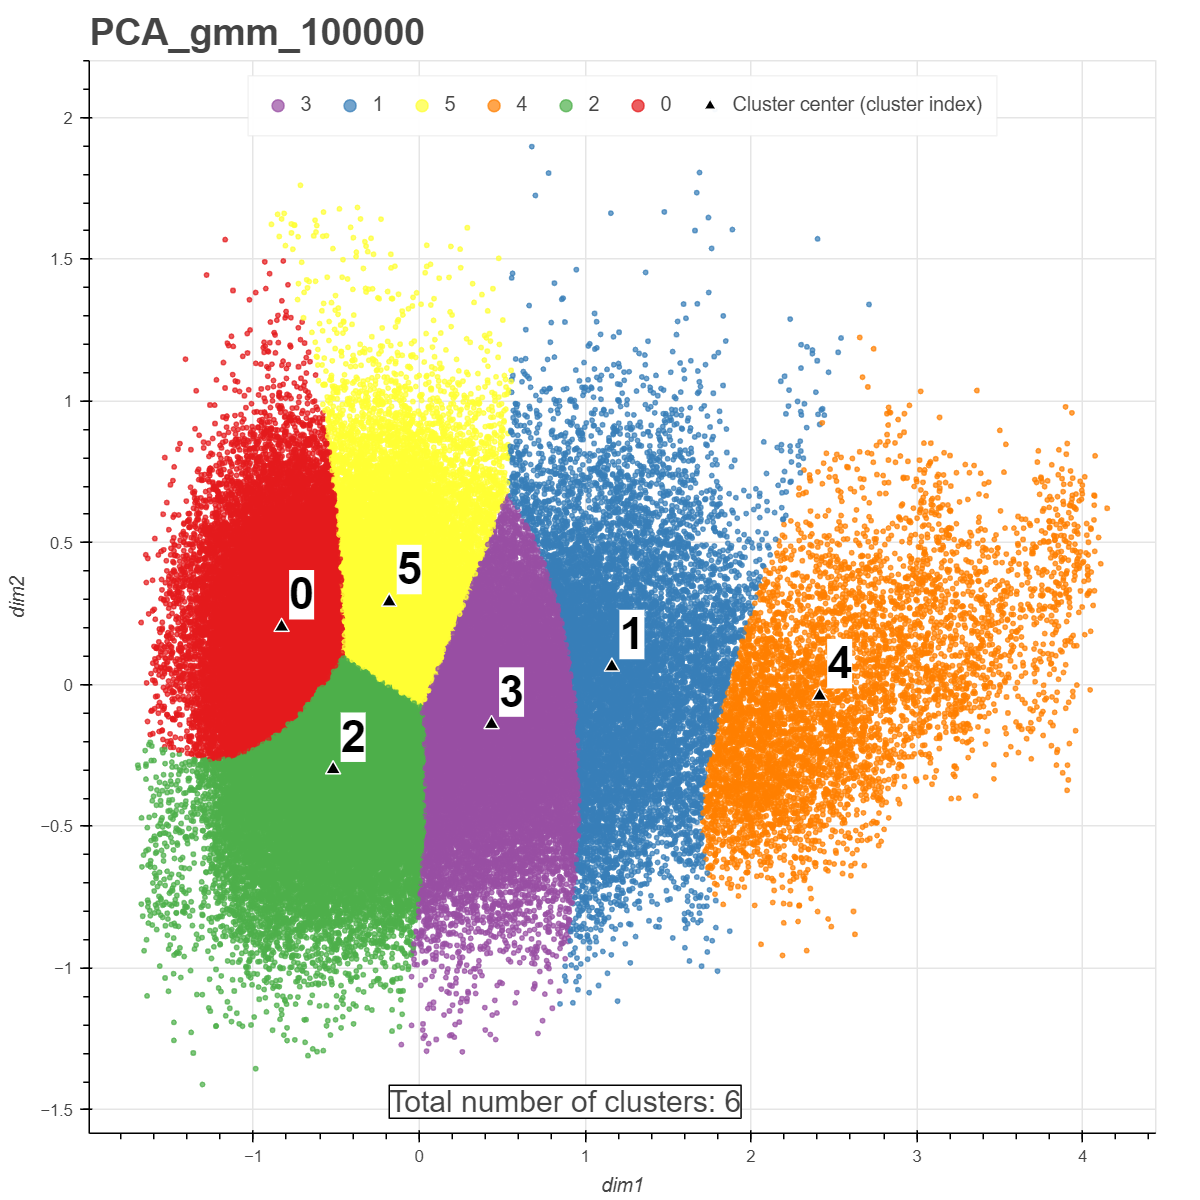
\includegraphics[width=.3\textwidth]{projects/Gustave_Li/Docs/pics/Clustering/Cluster_map/PCA_gmm.png}}
    \caption{Clustering results generated from PCA descriptors data, cluster num: 6}
    \label{fig: clustering PCA}
\end{figure}

\begin{figure}[H]
    \centering
    \subfloat[KMeans]{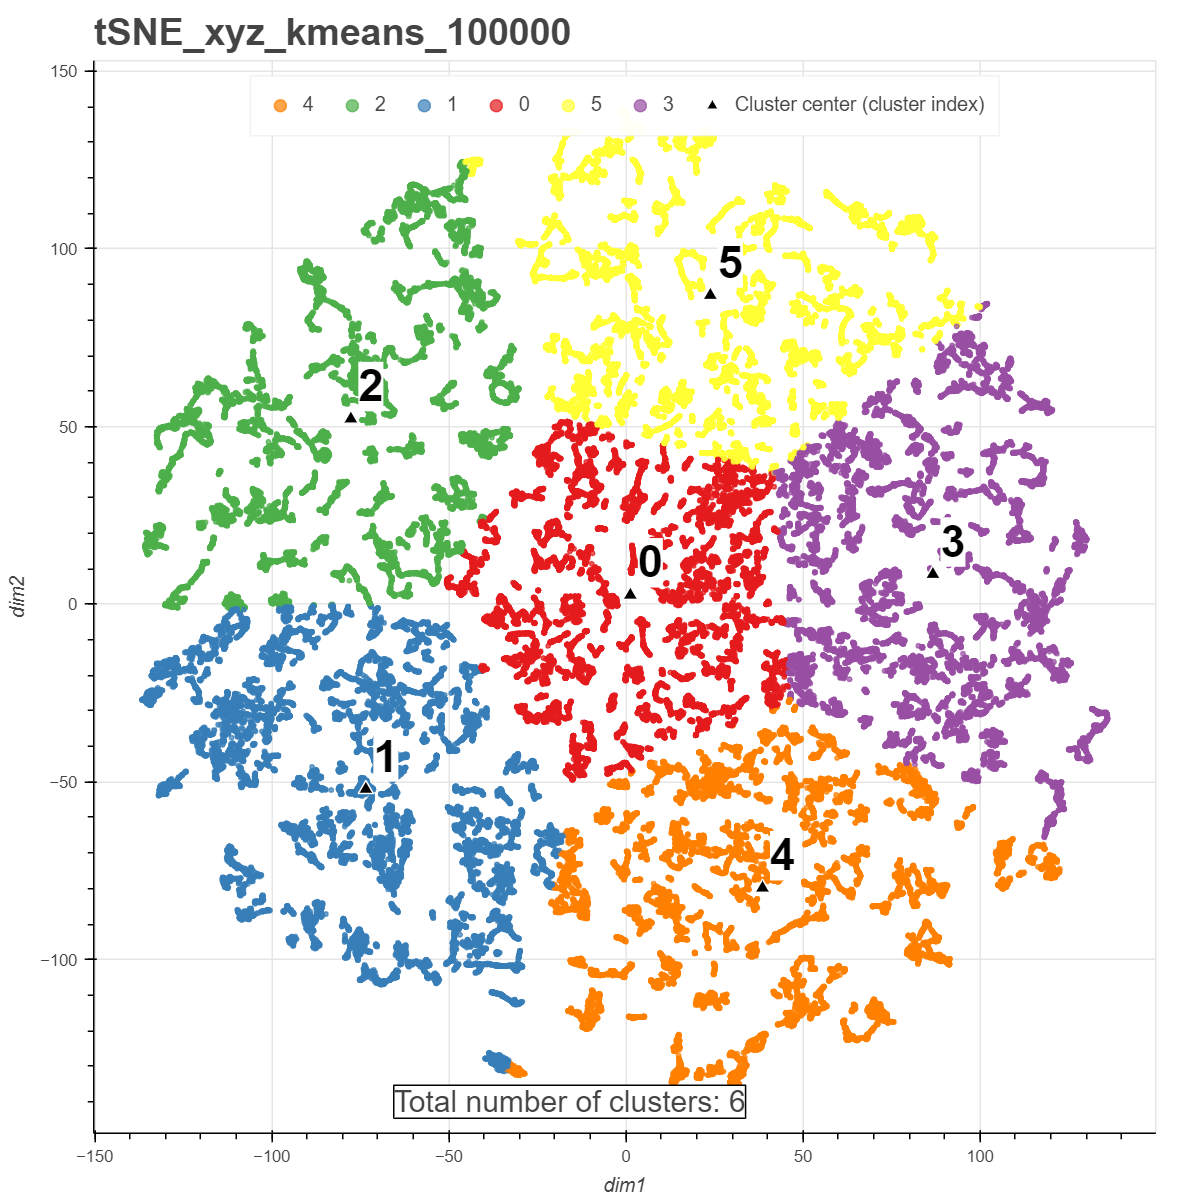
\includegraphics[width=.3\textwidth]{projects/Gustave_Li/Docs/pics/Clustering/Cluster_map/tsne_xyz_kmeans.png}}
    \subfloat[KMedoids]{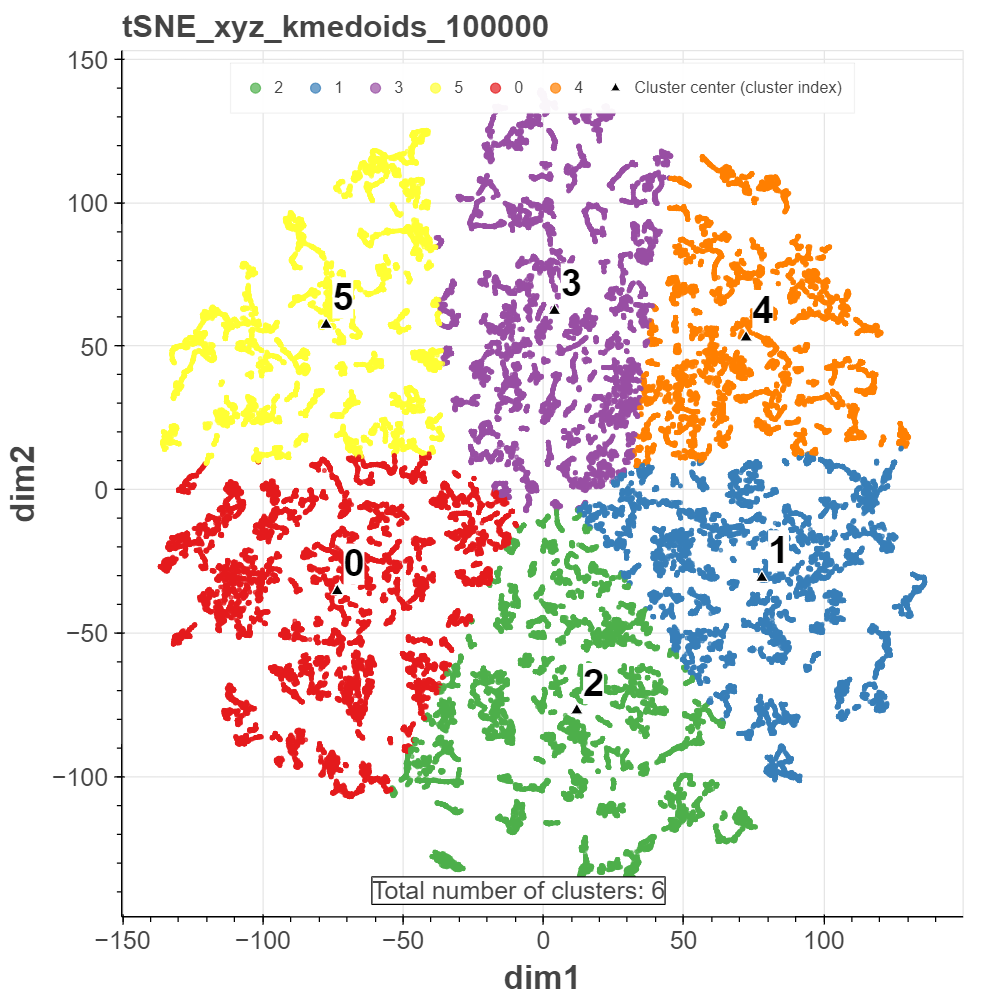
\includegraphics[width=.3\textwidth]{projects/Gustave_Li/Docs/pics/Clustering/Cluster_map/tsne_xyz_kmedoids.png}}
    \subfloat[GMM]{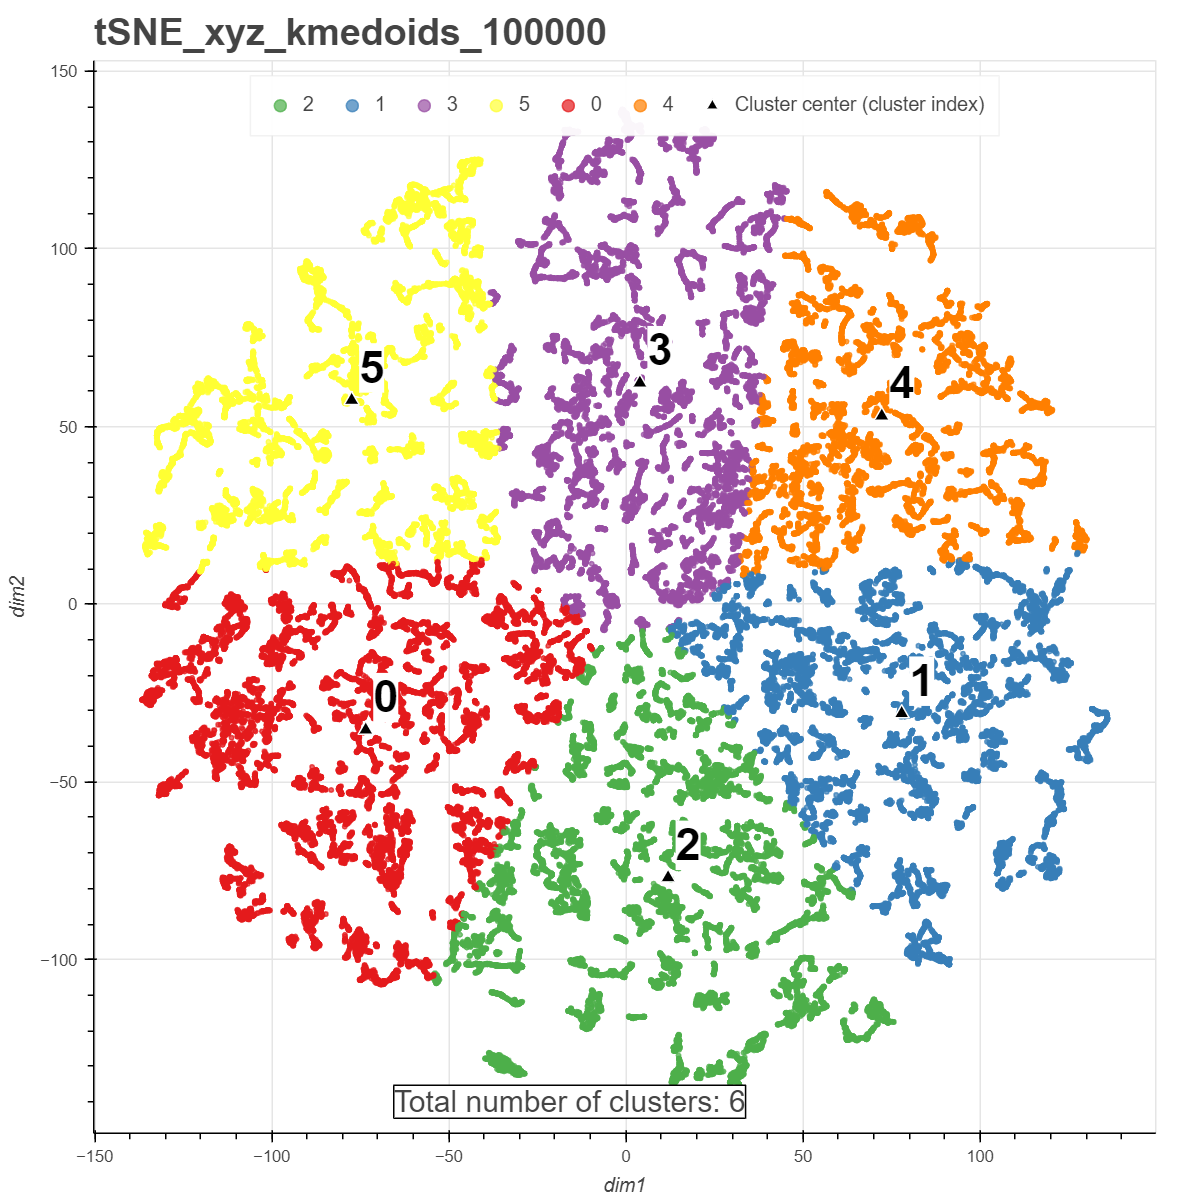
\includegraphics[width=.3\textwidth]{projects/Gustave_Li/Docs/pics/Clustering/Cluster_map/tsne_xyz_gmm.png}}
    \caption{Clustering results generated from tSNE xyz data, cluster num: 6}
    \label{fig: clustering tSNE}
\end{figure}

\subsubsection{Cluster Population}
Cluster population is another intuitive and critical method to evaluate clustering quality. Our aim is to find signature structures that represent its members, yet population of a cluster should be big enough to fulfill the need for representation. After inspection, it is defined that a meaningful cluster should have at least 5\% of the total population.

\begin{figure}[H]
    \centering
    \subfloat[ClusterNum:6]{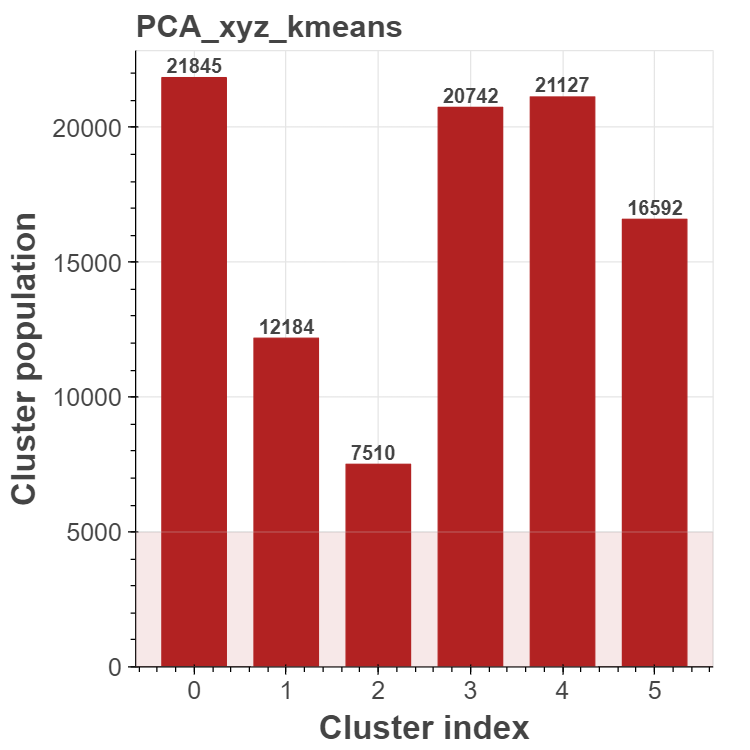
\includegraphics[width=.32\textwidth]{projects/Gustave_Li/Docs/pics/Clustering/Cluster_population/PCA_xyz_kmeans_6.png}}
    \subfloat[ClusterNum:7]{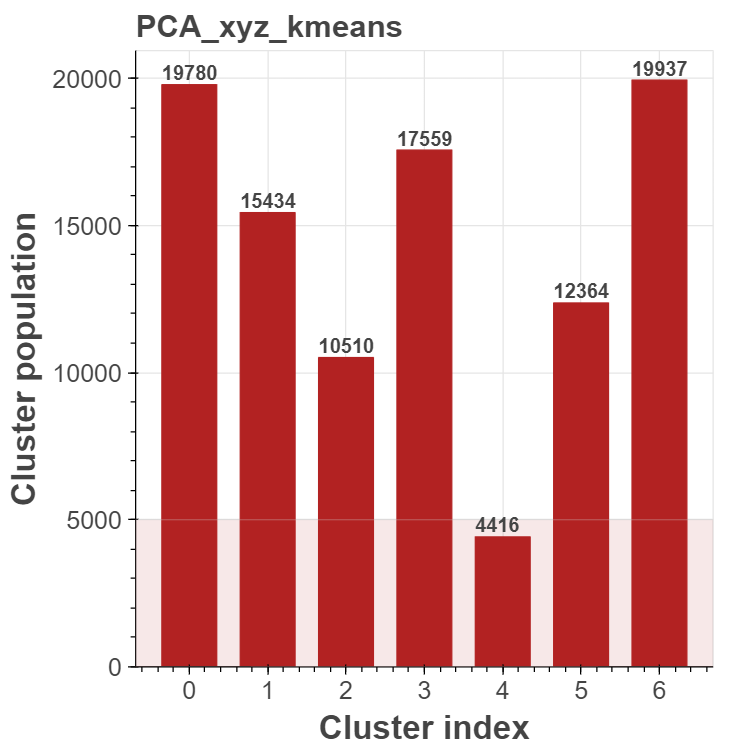
\includegraphics[width=.32\textwidth]{projects/Gustave_Li/Docs/pics/Clustering/Cluster_population/PCA_xyz_kmeans_7.png}}
    \subfloat[ClusterNum:8]{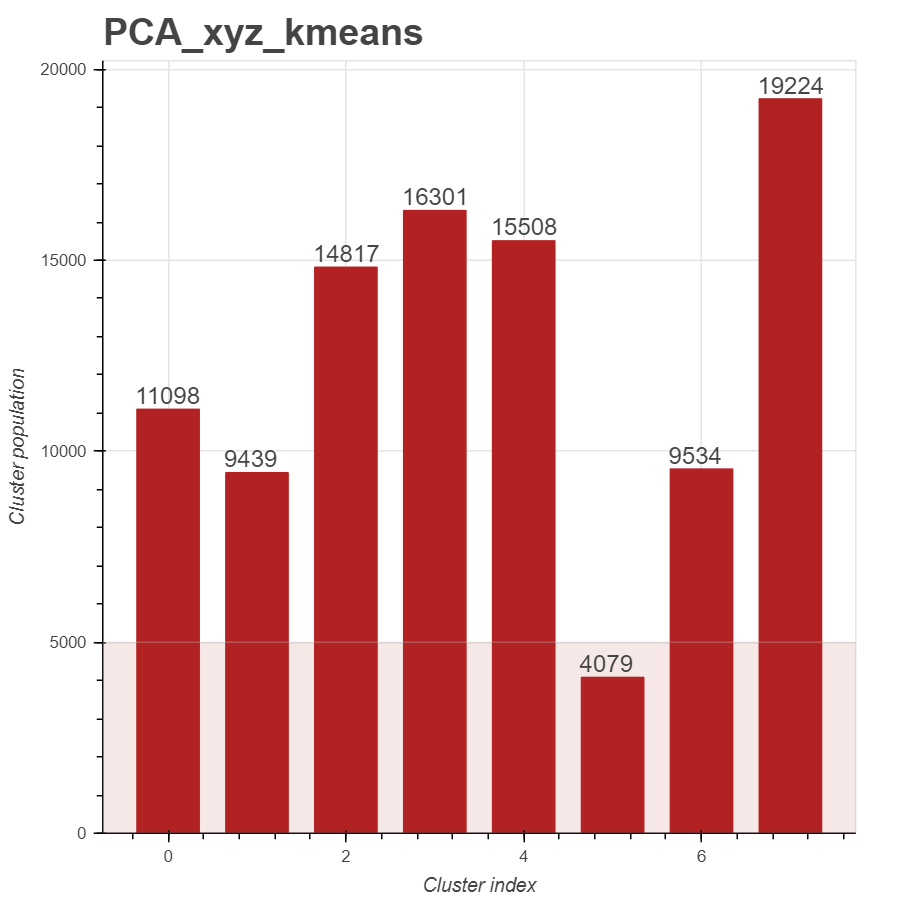
\includegraphics[width=.32\textwidth]{projects/Gustave_Li/Docs/pics/Clustering/Cluster_population/PCA_xyz_kmeans_8.png}}
    \caption{Clustering population generated from PCA\_xyz\_KMeans}
    \label{fig: clustering pop}
\end{figure}

A typical example was shown in Figure \ref{fig: clustering pop}. The 5\% box was plotted in light red, and the red bars representing population should be above the 5\% line. When the cluster number was set to 6, all the cluster population exceeded 5\%, indicating a meaningful clustering result. However, when cluster number rises, one of the cluster dropped below the 5\% line and it continued to decrease as more clusters was requested. This result revealed that an existing cluster was further split and merged with other clusters when the desired cluster number increased, making the cluster population smaller thus less representative. Accordingly, setting the cluster number to 7 or 8 may suffer from overfitting.

\subsubsection{Scoring}

\subsubsection{Pairwise RMSD \& Pearson Correlation}

\subsection{High-dimensioanl Clustering}

\subsubsection{Cluster Population}

\subsubsection{Cluster Map}

\section{Conclusion}


\pagebreak
\bibliographystyle{unsrt}
\bibliography{references.bib}

\end{document}